%----------------------------------------------------------------------------------------
% PACKAGES AND OTHER DOCUMENT CONFIGURATIONS
%----------------------------------------------------------------------------------------
\documentclass{article}
\usepackage{fancyhdr} % Required for custom headers
\usepackage{lastpage} % Required to determine the last page for the footer
\usepackage{extramarks} % Required for headers and footers
\usepackage[usenames,dvipsnames]{color} % Required for custom colors
\usepackage{graphicx} % Required to insert images
\usepackage{listings} % Required for insertion of code
\usepackage{courier} % Required for the courier font
\usepackage{lipsum} % Used for inserting dummy 'Lorem ipsum' text into the template
\usepackage[utf8]{inputenc}
\usepackage[ngerman]{babel}
% Margins
\topmargin=-0.45in
\evensidemargin=0in
\oddsidemargin=0in
\textwidth=6.5in
\textheight=9.0in
\headsep=0.25in
\linespread{1.1} % Line spacing
% Set up the header and footer
\pagestyle{fancy}
%\lhead{\hmwkAuthorName} % Top left header
\chead{\hmwkClass\ : \hmwkTitle} % Top center head
\rhead{\firstxmark} % Top right header
\lfoot{\lastxmark} % Bottom left footer
\cfoot{} % Bottom center footer
\rfoot{Page\ \thepage\ of\ \protect\pageref{LastPage}} % Bottom right footer
\renewcommand\headrulewidth{0.4pt} % Size of the header rule
\renewcommand\footrulewidth{0.4pt} % Size of the footer rule
\setlength\parindent{0pt} % Removes all indentation from paragraphs
%----------------------------------------------------------------------------------------
% CODE INCLUSION CONFIGURATION
%----------------------------------------------------------------------------------------
\definecolor{MyDarkGreen}{rgb}{0.0,0.4,0.0} % This is the color used for comments
\lstloadlanguages{Perl} % Load Perl syntax for listings, for a list of other languages supported see: ftp://ftp.tex.ac.uk/tex-archive/macros/latex/contrib/listings/listings.pdf
\lstset{language=Perl, % Use Perl in this example
frame=single, % Single frame around code
basicstyle=\small\ttfamily, % Use small true type font
keywordstyle=[1]\color{Blue}\bf, % Perl functions bold and blue
keywordstyle=[2]\color{Purple}, % Perl function arguments purple
keywordstyle=[3]\color{Blue}\underbar, % Custom functions underlined and blue
identifierstyle=, % Nothing special about identifiers
commentstyle=\usefont{T1}{pcr}{m}{sl}\color{MyDarkGreen}\small, % Comments small dark green courier font
stringstyle=\color{Purple}, % Strings are purple
showstringspaces=false, % Don't put marks in string spaces
tabsize=5, % 5 spaces per tab
%
% Put standard Perl functions not included in the default language here
morekeywords={rand},
%
% Put Perl function parameters here
morekeywords=[2]{on, off, interp},
%
% Put user defined functions here
morekeywords=[3]{test},
%
morecomment=[l][\color{Blue}]{...}, % Line continuation (...) like blue comment
numbers=left, % Line numbers on left
firstnumber=1, % Line numbers start with line 1
numberstyle=\tiny\color{Blue}, % Line numbers are blue and small
stepnumber=5 % Line numbers go in steps of 5
}
% Creates a new command to include a perl script, the first parameter is the filename of the script (without .pl), the second parameter is the caption
\newcommand{\perlscript}[2]{
\begin{itemize}
\item[]\lstinputlisting[caption=#2,label=#1]{#1.pl}
\end{itemize}
}
%----------------------------------------------------------------------------------------
% DOCUMENT STRUCTURE COMMANDS
% Skip this unless you know what you're doing
%----------------------------------------------------------------------------------------
% Header and footer for when a page split occurs within a problem environment
\newcommand{\enterProblemHeader}[1]{
%\nobreak\extramarks{#1}{#1 continued on next page\ldots}\nobreak
%\nobreak\extramarks{#1 (continued)}{#1 continued on next page\ldots}\nobreak
}
% Header and footer for when a page split occurs between problem environments
\newcommand{\exitProblemHeader}[1]{
%\nobreak\extramarks{#1 (continued)}{#1 continued on next page\ldots}\nobreak
%\nobreak\extramarks{#1}{}\nobreak
}
\setcounter{secnumdepth}{0} % Removes default section numbers
\newcounter{homeworkProblemCounter} % Creates a counter to keep track of the number of problems
\newcommand{\homeworkProblemName}{}
\newenvironment{homeworkProblem}[1][Problem \arabic{homeworkProblemCounter}]{ % Makes a new environment called homeworkProblem which takes 1 argument (custom name) but the default is "Problem #"
\stepcounter{homeworkProblemCounter} % Increase counter for number of problems
\renewcommand{\homeworkProblemName}{#1} % Assign \homeworkProblemName the name of the problem
\section{\homeworkProblemName} % Make a section in the document with the custom problem count
%\enterProblemHeader{\homeworkProblemName} % Header and footer within the environment
}{
%\exitProblemHeader{\homeworkProblemName} % Header and footer after the environment
}
\newcommand{\problemAnswer}[1]{ % Defines the problem answer command with the content as the only argument
\noindent\framebox[\columnwidth][c]{\begin{minipage}{0.98\columnwidth}#1\end{minipage}} % Makes the box around the problem answer and puts the content inside
}
\newcommand{\homeworkSectionName}{}
\newenvironment{homeworkSection}[1]{ % New environment for sections within homework problems, takes 1 argument - the name of the section
\renewcommand{\homeworkSectionName}{#1} % Assign \homeworkSectionName to the name of the section from the environment argument
\subsection{\homeworkSectionName} % Make a subsection with the custom name of the subsection
%\enterProblemHeader{\homeworkProblemName\ [\homeworkSectionName]} % Header and footer within the environment
}{
%\enterProblemHeader{\homeworkProblemName} % Header and footer after the environment
}
%----------------------------------------------------------------------------------------
% NAME AND CLASS SECTION
%----------------------------------------------------------------------------------------
\newcommand{\hmwkTitle}{Übung\ \#9} % Assignment title
\newcommand{\hmwkDueDate}{Mittwoch,\ 28.\ Januar\ 2015} % Due date
\newcommand{\hmwkClass}{Parallel Computer Architecture} % Course/class
\newcommand{\hmwkClassTime}{} % Class/lecture time
\newcommand{\hmwkClassInstructor}{} % Teacher/lecturer
\newcommand{\hmwkAuthorName}{Günther Schindler, Fabian Finkeldey, Shamna Shyju} % Your name
%----------------------------------------------------------------------------------------
% TITLE PAGE
%----------------------------------------------------------------------------------------
\title{
\vspace{2in}
\textmd{\textbf{\hmwkClass:\ \hmwkTitle}}\\
\normalsize\vspace{0.1in}\small{Abgabe\ am\ \hmwkDueDate}\\
\vspace{0.1in}\large{\textit{\hmwkClassTime}}
\vspace{3in}
}
\author{\textbf{\hmwkAuthorName}}
\date{} % Insert date here if you want it to appear below your name
%----------------------------------------------------------------------------------------
\begin{document}
\maketitle
%----------------------------------------------------------------------------------------
% TABLE OF CONTENTS
%----------------------------------------------------------------------------------------
%\setcounter{tocdepth}{1} % Uncomment this line if you don't want subsections listed in the ToC
\newpage
\tableofcontents
\newpage
%----------------------------------------------------------------------------------------
% Parallele Berechnung von Pi
%----------------------------------------------------------------------------------------
\begin{homeworkProblem}[Parallele Berechnung von Pi]
In der letzten Übung soll Pi mittels der Arkustangensreihe angenähert werden.
Die Parallelisierung soll mittels MPI und dem Master-Slave-Modell erfolgen.
\\\\
Für die Leistungsanalyse wurde die Ausführungszeit in Abhängigkeit der Genaugigkeit
visualisiert.
\begin{center}
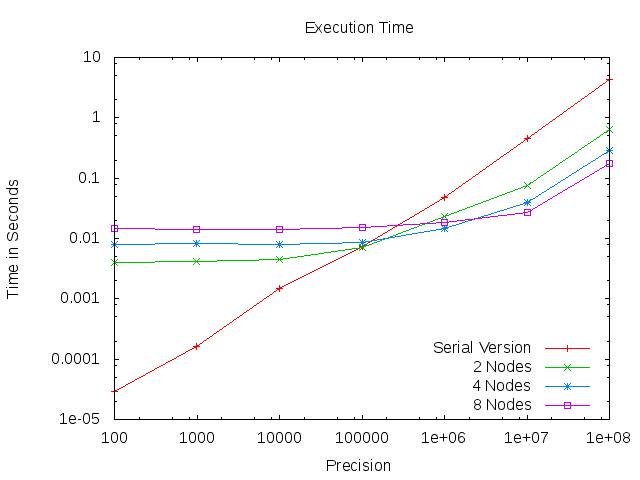
\includegraphics[width=0.7\columnwidth]{9.1/exec-time}
\end{center}
Die Grafik zeigt deutlich die benötigte Zusatzzeit um die Annäherung zu parallelisieren.
Für Genaugigkeiten unter $ 10^5 $ ist die sequentielle Version deutlich schneller.
Der Vorteil der parallisierten Variante wird erst für höhere Genaugigkeitein 
sichtbar. So können bei $ 10^8 $ Summanden mehrere Sekunden eingespart werden.
\\\\
Um den Vorteil der parallelen Version deutlich zu zeigen, wurde ebenfalls der 
resultierende Speed-Up in Abhängigkeit der Genaugigkeit visualisiert.
\begin{center}
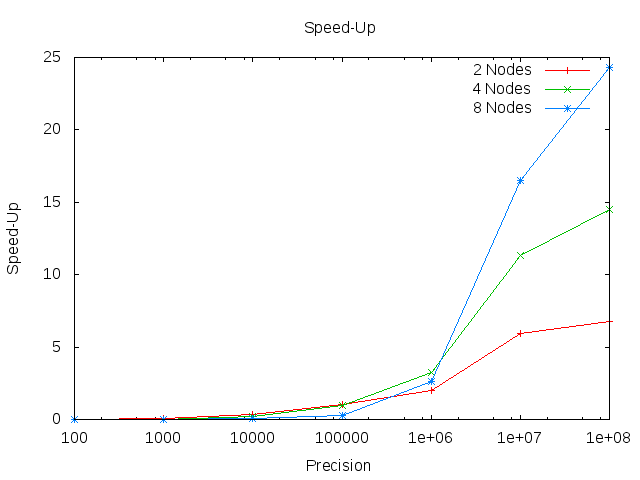
\includegraphics[width=0.7\columnwidth]{9.1/speed-up}
\end{center}
Es fällt auf, dass sich eine Parallelisierung erst ab einer Genaugigkeit von $ 10^6 $
lohnt. Danach können aber mit steigender Knotenanzahl deutliche Leistungssteigerungen
erzielt werden.
\end{homeworkProblem}

%----------------------------------------------------------------------------------------
% Auswertung - Hitzeverteilung revisited again (MPI)
%----------------------------------------------------------------------------------------
\begin{homeworkProblem}[Hitzeverteilung revisited again (MPI)]
Als nächstes sollte die Hitzeverteilung mit Hilfe von MPI parallelisiert werden. 

Für die Implementierung wurde ebenfalls das Master-Slave-Prinzip verwendet. Ein 
Thread, der Master-Thread, vollzieht eine 1D-Dekomposition des Grids (vgl. Abbildung)
und sendet die einzelnen Slices an die Slave-Threads.
\begin{center}
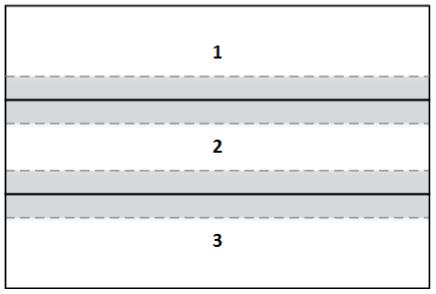
\includegraphics[width=0.5\columnwidth]{9.2/decomp}
\end{center}
Die Slave-Threads berechnen die einzelnen Slices für eine beliebige Anzahl an 
Iterationen/Steps, tauschen währenddessen die Halo-Elemente gegenseitig aus und 
senden ihre Ergebnisse zurück zum Master-Thread. Dieser fügt die einzelnen Slices
schließlich wieder zu einem vollständigen Grid zusammen.
\\\\
Bei der Leistungsanalyse wurden zunächst die möglichen Iterationen pro Sekunden in 
Abhängigkeit von den ausgeführten Iterationen/Steps ermittelt. Die Grid-Größe wurde
auf 1024x1024 gesetzt und die eingesetzten Threads variieren zwischen 1 und 16.
\begin{center}
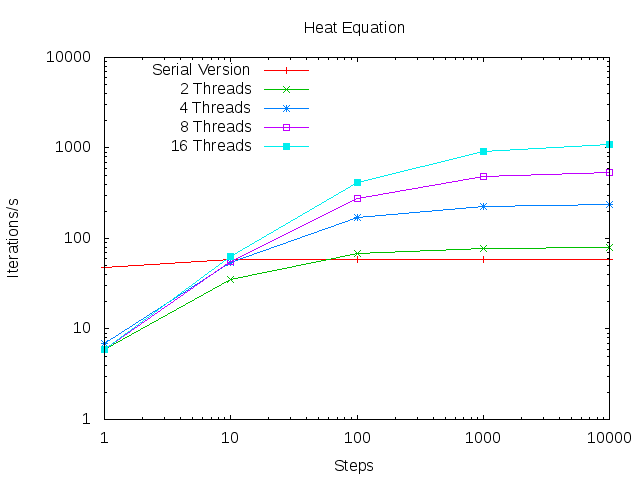
\includegraphics[width=0.7\columnwidth]{9.2/iterations}
\end{center}
Ähnlich wie bei der Pi-Annäherung hängt hier die Leistung auch wieder stark von der
Anzahl der Berechnungen ab. Die Grafik zeigt, dass sich eine Parallelisierung erst 
ab 10 Iterationen/Steps lohnt. Danach können jedoch, bei gleichbleibenden 59
Iterationen/s der sequentiellen Version, bis zu knapp 1000 Iterationen/s für 16
Threads erzielt werden.
\\\\
Betrachtet man den Verlauf des Speed-Up bestätigt sich diese Leistungsanalyse. 
\begin{center}
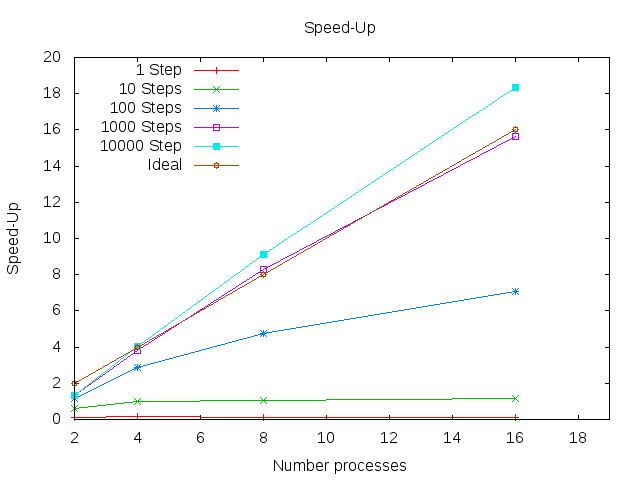
\includegraphics[width=0.7\columnwidth]{9.2/speed-up}
\end{center}
Je mehr Iterationen berechnet werden, desto besser ist die resultierende Leistung.
Bei 1.000 Iterationen bewegt sich der Speed-Up nahe am idealen Speed-Up. Für 10.000
Iterationen kann sogar ein superlinearer Speed-Up erreicht werden.
\end{homeworkProblem}

%----------------------------------------------------------------------------------------
% Fazit (Pthreads, OpenMP, MPI)
%----------------------------------------------------------------------------------------
\begin{homeworkProblem}[Fazit (Pthreads, OpenMP, MPI)]
Vergleicht man die drei Programmierkonzepte PThreads, OpenMP und MPI bezüglich des 
Arbeitsaufwandes, zeichnet sich klar OpenMP durch seine Einfachheit aus. An zweiter
Stelle befindet sich die Parallelisierung durch Pthreads. Pthreads sind ähnlich 
einfach einzusetzen, jedoch erfordert es hier mehr manuellen Aufwand im Vergleich zu
OpenMP. An letzter Stelle befindet sich der Einsatz von MPI. Das Message Pasing Interface
hat sich als hochgradig Arbeitsaufwändig herausgestellt.
\\\\
Der hohe Arbeitsaufwand bei MPI ist auf die Tatsache zurückzuführen, dass es für
Distributed Memory (bzw. Cluster-Systeme) hervorragend geeignet ist. Die Anforderung
von OpenMPI und Pthreads an Shared Memory lässt sie bezüglich der Leistung schnell 
an ihre Grenzen stoßen.
\\\\
Letztendlich lässt sich sagen, dass eine einfache, schnelle Parallelisierung für 
Shared Memory Systeme am besten mit OpenMP bzw. Pthreads realisieren lässt. Hat man 
hohe Leistungsanforderungen und ein Cluster System zur Verfügung, sollte jedoch
auf MPI zurückgegriffen werden.
\end{homeworkProblem}
\pagebreak

\end{document}
